\documentclass[a4paper,11pt]{report}
\usepackage[T1]{fontenc}
\usepackage[utf8]{inputenc}
\usepackage{lmodern}
\usepackage[spanish]{babel}
\usepackage{textcomp}
\usepackage{amsmath}
\usepackage{amsfonts}
\usepackage[framed,numbered,autolinebreaks]{mcode}
\usepackage{amssymb}
\usepackage{graphicx}
\usepackage{caption}
\usepackage{subcaption}
\usepackage{fancyhdr}
\usepackage{float}
\usepackage{color}
\usepackage[left=2cm,right=2cm,top=2cm,bottom=2cm]{geometry}

\title{Reporte 3 Práctica 4}
\author{Cabrera López Óscar Emilio}

\pagestyle{fancy}
\fancyhf{}
\lhead[]{}
\chead[]{}
\rfoot{\thepage}
\lfoot[]{}
\cfoot[]{}

\renewcommand\headrule
{{\color[RGB]{98,36,35}%
    \hrule height 2pt
    width\headwidth
    \vspace{1.3pt}%
    \hrule height 1pt
    width\headwidth
  }}
  \addto\captionsspanish{\def\tablename{Tabla}} %imprime Tabla en lugar de Cuadro
  %%
  \spanishdecimal{.}


\begin{document}
\thispagestyle{fancy}
\maketitle
\tableofcontents
\newpage
\setcounter{chapter}{1}

\section{Señal 1}
Señal senoidal
  \begin{figure}[H]
    \begin{center}
      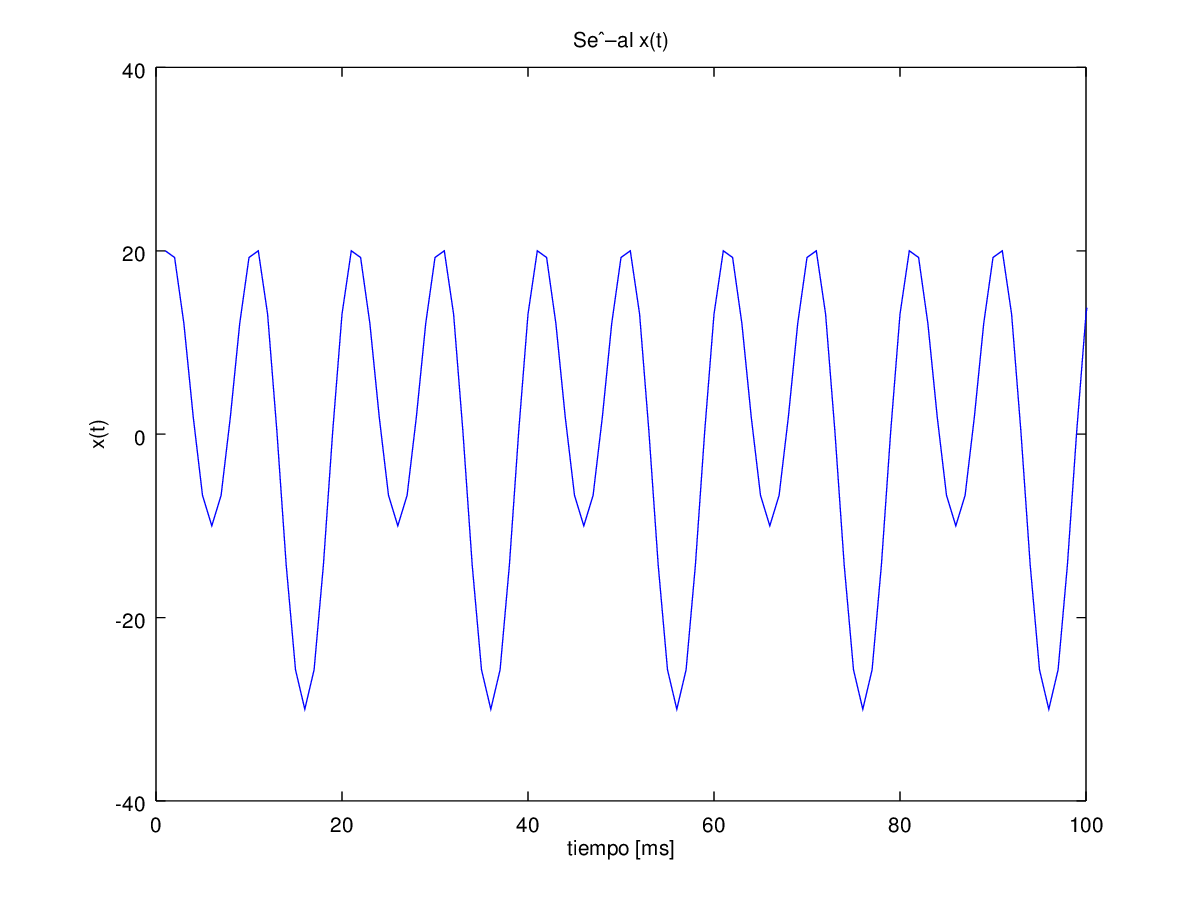
\includegraphics[width=0.6\textwidth]{./senal1}
      \caption{Diagrama de polos y ceros}
    \end{center}
  \end{figure}
  Código en Matlab:
  \lstinputlisting{./senal1.m}
\end{document}
